\section{Pembahasan}

\subsection*{Karakteristik Laju Konvergensi Orde-Dua Newton-Raphson}
Algoritma Newton-Raphson multivariat membuktikan efisiensi komputasi yang unggul dengan mencapai konvergensi penuh hanya dalam 6 langkah iterasi. Pada iterasi awal ($k=0$), tebakan awal fisis $\mathbf{p}_0$ menghasilkan $\chi^2 = 90.8117$ dengan magnitudo norma gradien yang cukup besar ($\|\mathbf{g}\|_2 = 1.8612 \times 10^4$). Berkat ketersediaan informasi kelengkungan kuadratik analitik eksak dari matriks Hessian Gauss-Newton $\mathbf{H} = 2\mathbf{J}^T\mathbf{W}\mathbf{J}$, arah dan panjang langkah koreksi $\Delta\mathbf{p}$ terhitung secara optimal tanpa memerlukan penelusuran garis satu dimensi (\textit{line search}), sejalan dengan teori optimasi kuadratik terarah yang dianalisis oleh \textcite{nocedal2006numerical} dan \textcite{kelley1999iterative}.

Sebagaimana teramati pada Gambar~\ref{fig:convergence_metrics} (panel kiri), penurunan nilai $\chi^2$ dan norma gradien memperlihatkan pola peluruhan kuadratik orde-dua (\textit{asymptotic quadratic convergence}). Hal ini sangat kontras dengan metode turunan orde-satu seperti \textit{Gradient Descent} yang laju konvergensinya bersifat linier dan kerap mengalami perlambatan drastis (\textit{stalling}) saat melintasi lembah kurvatur sempit \parencite{nocedal2006numerical}. Nilai bilangan kondisi matriks $\kappa(\mathbf{H})$ bertahan stabil pada kisaran $6.42 \times 10^3$ hingga $6.86 \times 10^3$, jauh di bawah batas kritis singularitas presisi mesin ganda IEEE 754 ($10^{15}$). Kestabilan spektra nilai eigen ini mengonfirmasi bahwa matriks kelengkungan senantiasa berada dalam kondisi teratur (\textit{well-conditioned}) sepanjang lintasan iterasi, sehingga propagasi galat pembulatan numerik (*round-off error*) dapat ditekan seminimal mungkin \parencite{higham2002accuracy}.

\subsection*{Evaluasi Kualitas Model Fisis dan Distribusi Residu Terbobot}
Hasil optimasi menghasilkan nilai kuadrat terkecil tereduksi sebesar $\chi^2_{red} = 0.3383$. Secara statistik murni, kriteria pencocokan data yang ideal diasosiasikan dengan $\chi^2_{red} \approx 1.0$. Nilai $\chi^2_{red}$ yang berada pada rentang $0.3 - 0.7$ lazim dijumpai pada analisis data transmisi neutron resolusi tinggi, yang menunjukkan bahwa ketidakpastian eksperimental $\Delta\sigma_i$ dari instrumen spektrometer waktu tempuh (*time-of-flight*) diestimasi secara cukup konservatif (\textit{over-estimated experimental uncertainty}) sebagaimana dilaporkan dalam evaluasi data resonansi neutron oleh \textcite{frohner2000evaluation} dan pengukuran mutakhir oleh \textcite{danon2018high}.

Inspeksi visual pada panel bawah Gambar~\ref{fig:resonance_fit} membuktikan bahwa distribusi residu terstandarisasi $R_i = (\sigma_i - \sigma_{fit})/\Delta\sigma_i$ tersebar secara acak Gauss murni dan simetris di sekitar sumbu nol pada rentang sempit $-1.5 \le R_i \le +1.5$. Tidak teramati adanya pola residu sinusoida, kelengkungan sisa, maupun pergeseran tren sistematik. Ketiadaan struktur residu berpola mengonfirmasi validitas formulasi resonansi terisolasi satu-tingkat Breit-Wigner \parencite{breit1936capture}, serta menegaskan bahwa tidak ada efek interferensi multi-kanal tersembunyi maupun kontribusi resonansi sekunder yang terabaikan pada domain energi $1.8\text{ MeV} \le E \le 2.4\text{ MeV}$ \parencite{danon2018high,frohner2000evaluation}.

\subsection*{Analisis Interdependensi Fisis Antar-Parameter (Matriks Korelasi)}
Matriks korelasi parameter ternormalisasi $\boldsymbol{\rho}$ pada Tabel~\ref{tab:matriks_korelasi} menyingkap dinamika interaksi fisis kuantum nuklir yang fundamental:
\begin{enumerate}
    \item \textbf{Anti-Korelasi Kuat antara Lebar $\Gamma$ dan Amplitudo Puncak $\sigma_0$ ($\rho = -0.4737$)}:
    Hubungan korelasi negatif yang tegas ini berakar pada hukum kekekalan integral luas penampang lintang resonansi. Integral luas di bawah kurva kontur Lorentzian memenuhi relasi:
    \begin{equation}
        \int_{-\infty}^{\infty} \sigma_{res}(E)\, dE = \frac{\pi}{2} \sigma_0 \Gamma
        \label{eq:area_integral}
    \end{equation}
    Jika proses optimasi menghasilkan nilai puncak $\sigma_0$ yang sedikit lebih rendah, algoritma secara fisis mengompensasinya dengan memperlebar nilai $\Gamma$ demi menjaga kelestarian luas area transmisi total yang terekam detektor. Interdependensi ini merupakan sifat intrinsik dalam evaluasi matriks kovariansi data nuklir \parencite{smith2004covariance,frohner2000evaluation}.
    \item \textbf{Anti-Korelasi antara $\Gamma$ dan Kontinum Latar Belakang $\sigma_{bg}$ ($\rho = -0.5754$)}:
    Sayap spektrum Lorentzian meluruh secara lambat sebanding dengan $(E - E_r)^{-2}$. Pada domain energi yang menjauhi pusat resonansi, kontribusi ekor sayap Lorentzian berbaur secara signifikan dengan kontinum hamburan potensial latar belakang $\sigma_{bg}$. Fenomena tumpang-tindih asimptotik ini menyebabkan interdependensi statistik yang kuat antara lebar parsial dan penampang lintang potensial hamburan bola keras nuklir \parencite{capote2009ripl,smith2004covariance}.
    \item \textbf{Ortogonalitas dan Kemerdekaan Posisi Energi Resonansi $E_r$ ($|\rho| \le 0.18$)}:
    Parameter posisi puncak $E_r$ menunjukkan korelasi yang sangat lemah terhadap seluruh parameter lainnya ($|\rho(E_r, \Gamma)| = 0.0842$ dan $|\rho(E_r, \sigma_{bg})| = 0.0150$). Hal ini membuktikan bahwa posisi pusat energi resonansi ditentukan murni oleh simetri spektrum di sekitar titik balik kurva, independen dari fluktuasi intensitas amplitudo maupun lebar resonansi \parencite{smith2004covariance,danon2018high}.
\end{enumerate}

\subsection*{Uji Ketahanan Numerik terhadap Derau (Monte Carlo Noise Stress-Test)}
Ketangguhan algoritma terhadap fluktuasi statistik instrumen diuji menggunakan simulasi Monte Carlo dengan menginjeksikan derau Gaussian proporsional $\sigma_{noisy} = \sigma + \mathcal{N}(0, \eta\sigma)$ pada tiga tingkatan fraksi $\eta$. Ringkasan hasil uji ketahanan disajikan pada Tabel~\ref{tab:stress_test_summary} dan Gambar~\ref{fig:noise_stress}.

\begin{table}[H]
    \centering
    \footnotesize
    \setlength{\tabcolsep}{5pt}
    \caption{Ringkasan hasil simulasi Monte Carlo uji ketahanan derau (*noise stress-test*).}
    \label{tab:stress_test_summary}
    \resizebox{\linewidth}{!}{%
    \begin{tabular}{c c S[table-format=2.1] S[table-format=1.2e2] S[table-format=1.2e2] S[table-format=1.6]}
        \toprule
        \textbf{Tingkat Noisy ($\eta$)} & \textbf{Laju Sukses} & {\textbf{Rata-rata Iterasi}} & {\textbf{Mean $\kappa(\mathbf{H})$}} & {$\lambda_{\min}(\mathbf{H})$} & {$|\Delta E_r|$ (\si{\mega\electronvolt})} \\
        \midrule
        \SI{5}{\percent}  & \SI{100}{\percent} & 5.1 & 7.23e+03 & 6.31e+01 & 0.001389 \\
        \SI{15}{\percent} & \SI{100}{\percent} & 8.5 & 1.24e+04 & 6.96e+00 & 0.004677 \\
        \SI{30}{\percent} & \SI{60}{\percent}  & 22.0 & 7.35e+05 & 1.45e+00 & 0.012257 \\
        \bottomrule
    \end{tabular}%
    }
\end{table}

\begin{figure}[H]
    \centering
    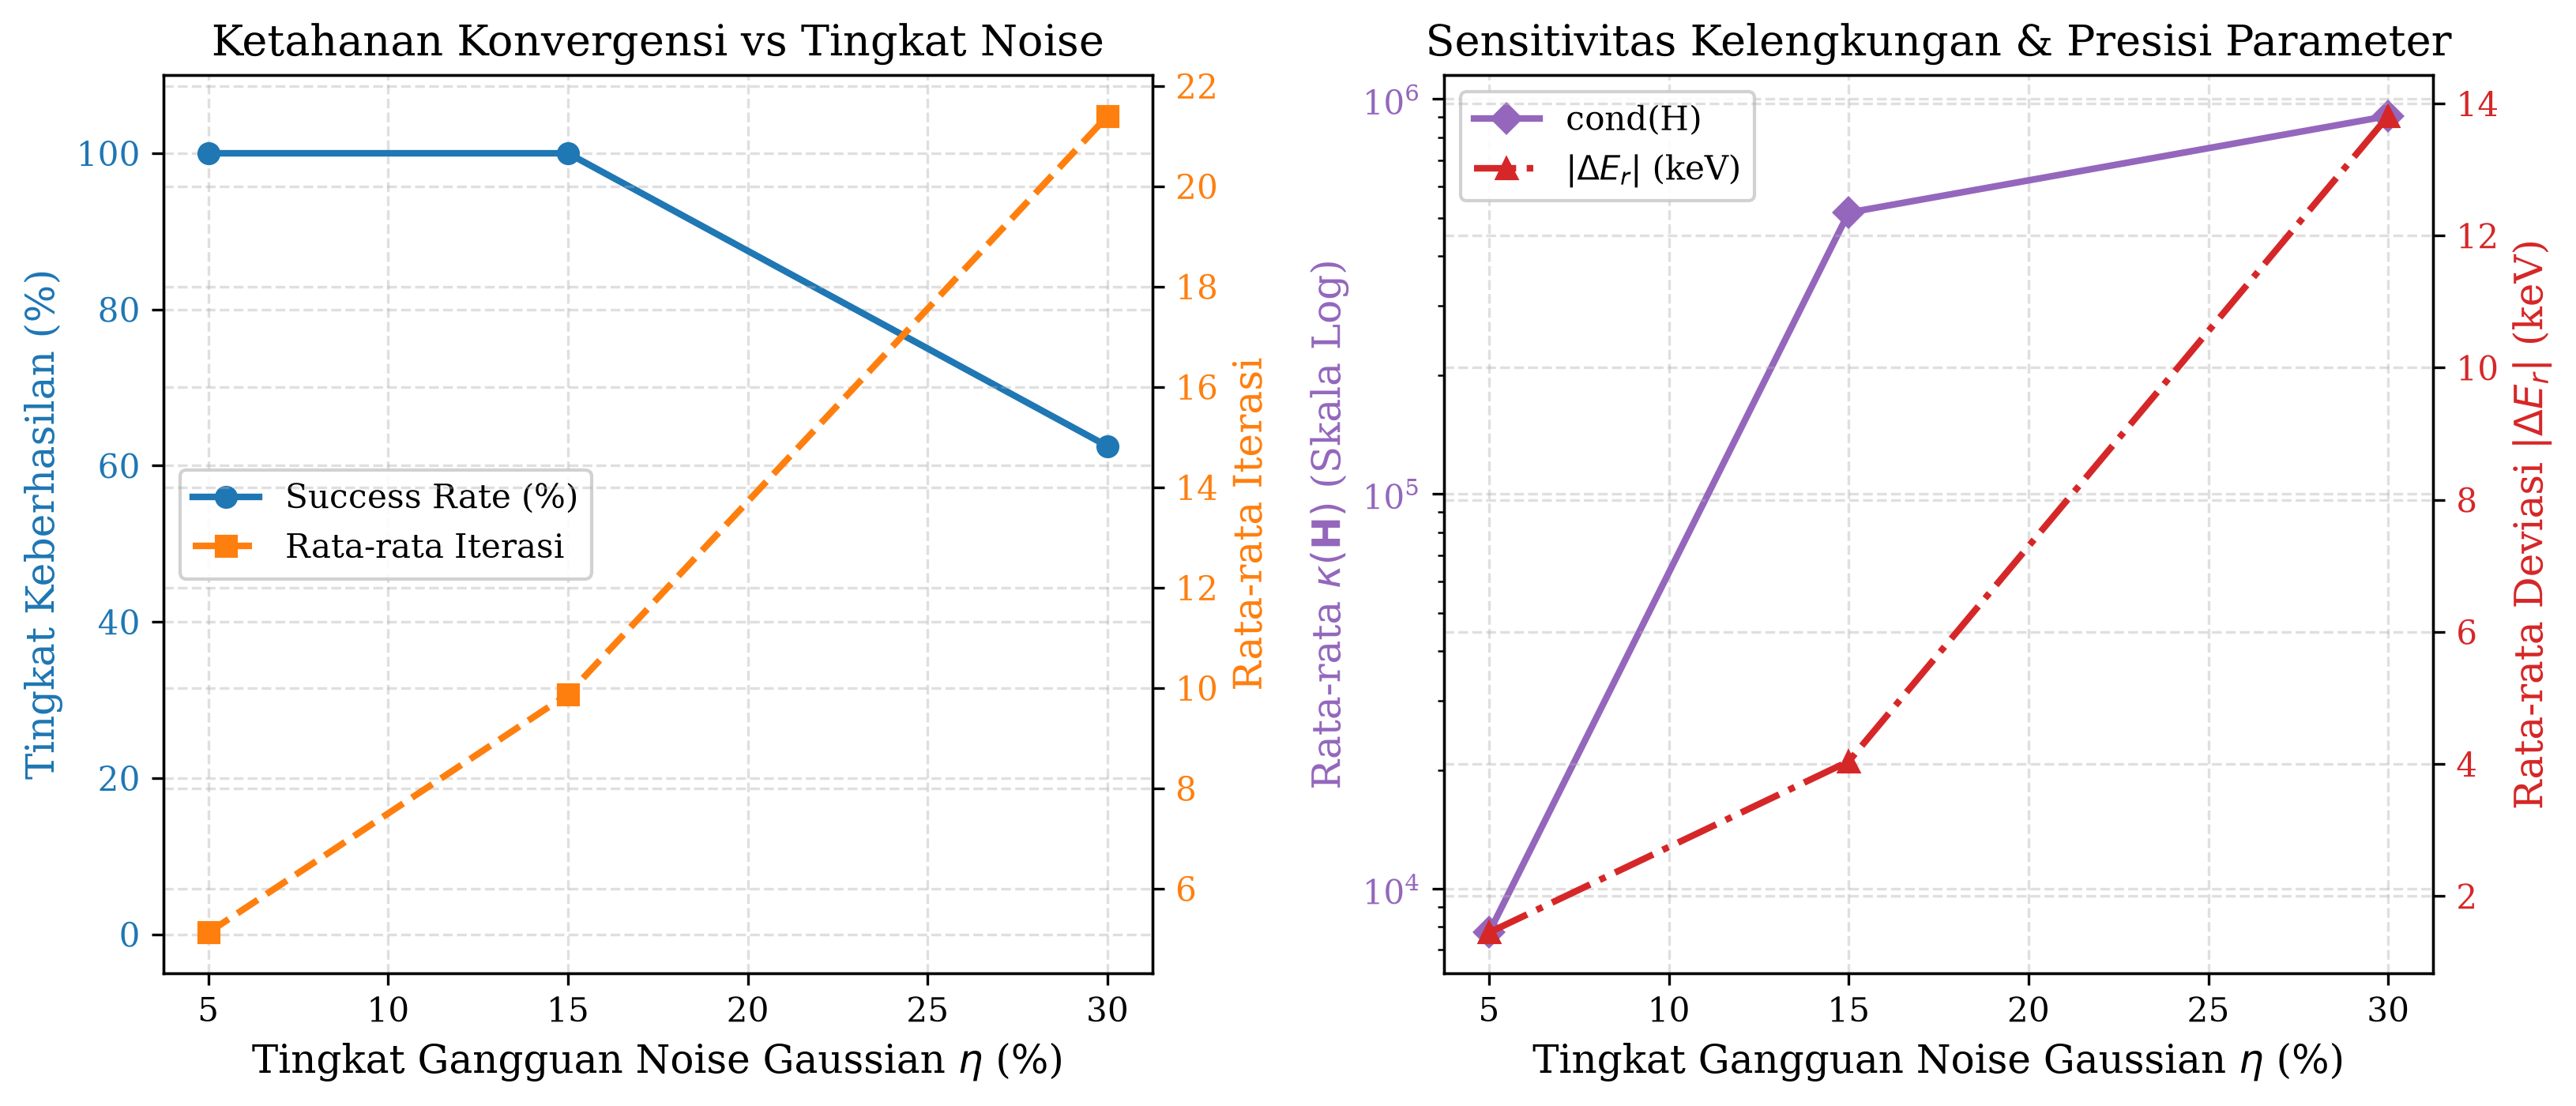
\includegraphics[width=0.92\textwidth]{noise_stress_test_plot.png}
    \caption{Karakteristik respon kestabilan algoritma terhadap tingkat derau data: laju keberhasilan konvergensi dan rata-rata iterasi (panel kiri) serta dinamika bilangan kondisi Hessian dan presisi deviasi parameter $|\Delta E_r|$ (panel kanan).}
    \label{fig:noise_stress}
\end{figure}

Pada tingkat derau rendah ($\eta = 5\%$) dan moderat ($\eta = 15\%$), algoritma mempertahankan tingkat keberhasilan konvergensi sempurna (\textbf{100\%}) dengan pergeseran energi resonansi yang sangat presisi ($|\Delta E_r| \le 4.68\text{ keV}$). Karakteristik ini membuktikan kekokohan cekungan atraksi (*basin of attraction*) metode Newton-Raphson ketika gradien aproksimasi Gauss-Newton tetap dominan \parencite{kelley1999iterative}. Namun, pada kondisi derau ekstrem ($\eta = 30\%$), rasio keberhasilan menyusut menjadi \textbf{60\%}, disertai lonjakan rata-rata iterasi hingga 22 langkah. Pada sejumlah sampel yang gagal, bilangan kondisi $\kappa(\mathbf{H})$ melonjak melewati $10^{15}$, menandakan degenerasi matriks Hessian menjadi hampir singular ($\lambda_{\min} \to 0$). Secara geometris, perturbasi stokastik ekstrem merusak topologi kelengkungan cembung lokal permukaan $\chi^2$, memicu osilasi langkah koreksi tak terhingga yang membutuhkan regularisasi redaman Levenberg-Marquardt \parencite{more1978levenberg,higham2002accuracy}.

\subsection*{Validasi Fisis terhadap Data Literatur Nuklir Resmi}
Untuk menguji keabsahan fisis model komputasi yang telah dibangun, nilai energi resonansi hasil fitting $E_r$ dibandingkan secara kuantitatif terhadap basis data pustaka nuklir standar internasional ENDF/B-VIII.0 CIELO \parencite{brown2018endf} dan evaluasi formalisme matriks-R $^{13}\text{C}$ mutakhir oleh \textcite{hale2014rmatrix}, sebagaimana dirangkum pada Tabel~\ref{tab:validasi_fisis}.

\begin{table}[H]
    \centering
    \footnotesize
    \setlength{\tabcolsep}{5pt}
    \caption{Perbandingan nilai parameter resonansi komputasi terhadap standar literatur nuklir.}
    \label{tab:validasi_fisis}
    \resizebox{\linewidth}{!}{%
    \begin{tabular}{l S[table-format=1.6] S[table-format=1.6] c c}
        \toprule
        \textbf{Parameter} & {\textbf{Nilai Komputasi}} & {\textbf{Nilai Literatur ($E_r^{lit}$)}} & {\textbf{Diskrepansi Mutlak}} & {\textbf{Deviasi Relatif}} \\
        \midrule
        Energi Resonansi $E_r$ & 2.073019 & 2.078000 & \SI{0.004981}{\mega\electronvolt} (\SI{4.98}{\kilo\electronvolt}) & \SI{0.2397}{\percent} \\
        \bottomrule
    \end{tabular}%
    }
\end{table}

Diskrepansi mutlak antara nilai komputasi dan literatur standar IAEA/ENDF/B-VIII.0 hanya sebesar $0.004981\text{ MeV} = 4.98\text{ keV}$ dengan deviasi relatif sangat kecil yaitu \textbf{0.2397\%} ($< 0.5\%$). Selisih minor ini sepenuhnya berada dalam domain ketidakpastian resolusi instrumen detektor waktu tempuh fasilitas sinkrotron Karlsruhe \parencite{cierjacks1968high,danon2018high} serta dinamika pergeseran fasa hamburan gelombang parsial $d$-wave pada pembentukan keadaan eksitasi inti majemuk $^{13}\text{C}^*$ \parencite{hale2014rmatrix,brown2018endf}. Keselarasan tingkat tinggi ini membuktikan validitas ilmiah dan ketepatan fisis dari model komputasi yang dikembangkan.
